\documentclass{l3proj}
\begin{document}

\title{Event sourcing as a microservices architecture}
\author{Connor Jardine \\
        David Wood \\
        Frank Bojen \\
        Naji Shehab \\
        Patrick Menlove}
\date{17 January 2018}
\maketitle

\begin{abstract}
This report presents a case study covering the implementation of an event-sourced application composed of microservices and an event bus. Built for Avaloq \cite{avaloq}, a Swiss company that builds software for banks, the application architecture is intended to enable exploration of any associated problems and solutions. Throughout this report, various architectural issues - such as maintaining consistency in a distributed system, enabling correlation of related events and enabling inter-service communication - will be discussed. Implementation-specific issues are also discussed, such as the practicality, advantages and disadvantages of developing the event bus in Rust.
\end{abstract}
\educationalconsent

\newpage
%------------------------------------------------------------------------------
\tableofcontents

\newpage
%------------------------------------------------------------------------------
\section{Introduction}
\label{sec:introduction}
This paper presents a case study of the advantages and disadvantages of event sourcing as a architecture for a microservices-based financial application - it will discuss the architectural challenges faced such as consistency in a distributed system; correlation of related events from different sources and reliability in highly asynchronous systems.

Further, this case study will discuss the technical hurdles specific to this implementation, in particular: the advantages and disadvantages of using the technologies used - Rust and React - in building the system and the benefits of quick deprecation and replacement of existing infrastructure for improvements.

The rest of the case study is structured as follows: a background on the requirements of the project; a deep-dive into the software development process and methodologies used; how consistency and correlation were designed and implemented; an overview of the improvements to service reliability brought on by implementation of the sticky round robin and acks; challenges in achieving persistence with couchbase and working with microservices; the design and implementation of the UI backend; and advantages and disadvantages of the core technologies used.

%==============================================================================
\section{Case Study Background}
\label{sec:background}
This project was completed on behalf of Avaloq. Avaloq is a Swiss company that specializes in the creation of bespoke software for banks and other customers in the financial industry. Avaloq serves over 450 financial institutions worldwide and their software underpins \$4 trillion globally.

Avaloq wanted a proof-of-concept event sourcing platform that would allow for the replay and distribution of arbitrary events across multiple subscribed services. In order to demonstrate this it was requested that a simple financial application capable of money transfers be created, consisting of at least three microservices communicating around a core event bus.

Event sourcing is an architecture where unlike traditional architectures the state of objects is not persisted, instead the sequence of events which created that state are. Event sourcing has numerous benefits:

\begin{itemize}
    \item State of any event bus client can be rebuilt entirely from the events.
    \item The application state can be inspected for any point in time by composing the events up until that time. This has major benefits for auditing.
\end{itemize}


Within the requested demo application, clients should be able to subscribe and publish events to the platform.

\begin{itemize}
    \item Subscribers and publishers need not be on the same machine.
    \item Subscribers should only receive events that interest them.
    \item Events should be generic in that they can represent any textual data.
    \item Events should be persistent and immutable.
\end{itemize}

It is also requested that a user-facing client that interacts with the three microservices be created.

%==============================================================================
\section{Process}
\label{sec:process}
Write something here!

\subsection{Pair Programming}
Write something here!

\subsection{Mentored Issues}
Write something here!

From the perspective of the mentor - mentored issues allow for a balance between providing too much assistance and allowing the mentee to do some research and learn by doing. It is also beneficial as it doesn't require meetings between the team members that can be hard to schedule.

\subsection{Learning Curves}
Write something here!

\subsection{Agile and Team Roles}
Write something here!

%==============================================================================
\section{Consistency}
\label{sec:consistency}

One of the fundamental challenges when building distributed systems is ensuring consistency - this is a challenge faced regardless of whether the system is built with an event sourced, modern three tier, sharded, lambda or streaming architecture.

Without an approach to handle consistency, distributed systems will run into a variety of problems. In this implementation specifically, it is desirable that the event bus has no insight into the events it is processing, this introduces further difficulties to any desirable solution.

The primary issue resulting from a lack of consistency in a distributed system is that two clients can mutate the same state simultaneously.

A traditional example of a problem related to consistency is double-spending. While double-spending is typically associated with digital currencies, it applies to many distributed systems and describes the state becomes inconsistent between participating nodes.

In the context of this event sourcing platform, there are multiple potential issues that could result of poor consistency:

\begin{itemize}
    \item It is important that a malicious or poorly implemented client cannot send events that would spend the same £5 from one end-user's balance multiple times.
    \item It is also important that if two events are sent they are received in the same order by all clients, this stops any given end-user from being mistakenly overdrawn if a client receives a withdrawal event before a deposit event.
\end{itemize}

Any solution for this problem must depend on the protocol for sending events, since the content of any given event cannot be known to the event bus.

Ensuring consistency is inherently a trade-off with speed, this will become evident as this paper discusses the various approaches that were considered for the event bus.

\subsection{Blockchain-Inspired Approach}
Initially, a blockchain-inspired was chosen. The blockchain \cite{blockchain} is a data structure that originates from Bitcoin \cite{bitcoin}, a digital crypto-currency, inspired by existing data structures like Merkle Trees \cite{merkletree}.

Blockchains are similar to singly linked lists except that contained in each node is the hash of the previous node, thereby enforcing an immutability of all nodes before the head of the list. Bitcoin builds on this by introducing a proof-of-work system so that the next head node can be chosen without the need for a centralized authority - this isn't required in the event bus implementation given that the event bus can act as a centralized authority.

The initial approach conceived was for each event to contain the hash of the previous event, enforced by the event bus.

\begin{figure}[ht]
\begin{center}
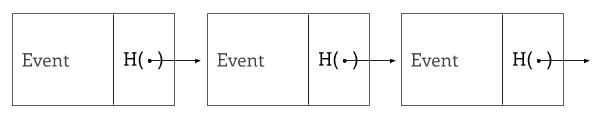
\includegraphics[width=15cm]{figures/consistency-1}
\end{center}
\caption{Blockchain-inspired Approach}
\label{fig:consistency-1}
\end{figure}


When an event was received that contained a hash that did not match the previous event expected by the event bus, then it would be rejected, and the client would be sent an rejection message containing the correct, expected hash. By including the expected hash in the rejection message, this implementation would still allow clients to successfully submit new events while not listening to all events.

One issue with this proposed approach is that a client that listens for \texttt{PendingTransaction} events might still have many queued to process and that despite having the correct next hash (from a rejection or through peeking at the queue) could produce a new event that contradicts one of the events still queued.

\subsection{Blockchain-Inspired with a Sequence Number}
In order to remedy this, inclusion of a sequence value per event type was proposed. This value would not be sent to clients with the hash on rejection and would therefore require that a client register for and process all events of that type in order to have the correct value.

The sequence value provided would start at zero for any given event type and be incremented by one for any subsequent event of that type.

\begin{figure}[ht]
\begin{center}
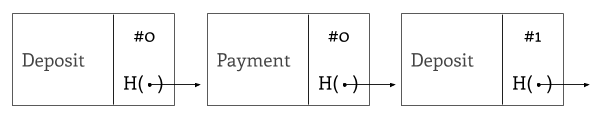
\includegraphics[width=15cm]{figures/consistency-2}
\end{center}
\caption{Blockchain-inspired with a Sequence Number}
\label{fig:consistency-2}
\end{figure}

This however would not solve the largest issue with a blockchain-esque approach, by enforcing a global ordering, if N events were sent simultaneously, then there would be a minimum of N! rejections and therefore could cause the event bus to be very slow in processing events.

\subsection{Sequence Key/Value Approach}
Building on the inclusion of a sequence number, the most recent solution to this problem involves the inclusion of both a sequence key and a sequence value - but no hash. A sequence key would be used to uniquely identify any events that could conflict. For example, in the context of a financial application, an account number could be used as a sequence key as any events that modify the state of an account should depend on the most recent state of that account.

\begin{figure}[ht]
\begin{center}
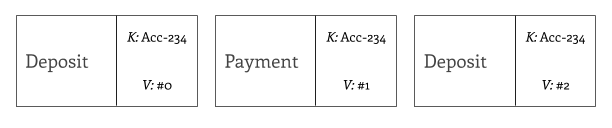
\includegraphics[width=15cm]{figures/consistency-3}
\end{center}
\caption{Sequence Key/Value}
\label{fig:consistency-3}
\end{figure}

In this scheme, the sequence value would function similarly to before, however, the sequence value would be incremented for each subsequent event of the same key rather than by event type.

%==============================================================================
\section{Correlation}
\label{sec:correlation}

Another required feature of the event bus implementation is the ability to trace units of work throughout the system. A unit of work consists of multiple events that when combined represent a single state change. An example of this would be a \texttt{PendingTransaction} that produces a \texttt{ConfirmedTransaction} or \texttt{RejectedTransaction} event.

\subsection{Correlation Tracking}
Implementation of correlation tracking involved modification of the event bus' client library to include a GUID which each event. However, if an event is related to a previous event and that previous event was provided, the correlation id of that event will be used instead of generating a new id.

\subsection{Session Tracking}
In addition to correlation tracking, this implementation also includes session tracking which can be used link all events produced by a given instance of a service. This could be useful if a bug was introduced into a microservice and it was desirable to find which events it produced during this time.

%==============================================================================
\section{Sticky Round Robin}
\label{sec:sticky-round-robin}

In the spirit of microservices, it is a requirement that multiple instances of a given service be able to run simultaneously in order to horizontally scale the processing performed by that service.

For this to be supported in the event bus implementation presented by this paper, it is required that a solution be developed that allows for this functionality while working within the constraints defined by the consistency solution.

\subsection{A naive approach}
A naive approach would be to allow many instances of a given service to connect without any functionality in the event bus to support this. However, this approach would be prone to problems.

In this scenario, the event bus would send any given event to all connected clients. If there were multiple instances of a service running, then both services would receive the event and begin processing - this could result in duplicate events being produced as a result - at best, this would waste processing power; at worst this effect could multiply (more duplicate events being processed more than once producting more duplicate events) and act as a denial of service the event bus.

\subsection{Round robin approach}
Initially, a round robin approach was considered, where clients would register which type of service they represent. Then, when an event is to be sent to a service type, the event bus would perform a round robin selection on the clients of that type. ie. It would cycle through each client.

One theorized issue with this solution is in the interaction with the consistency implementation. If events with the same consistency key are sent to many different clients then none of them will be able to keep track of the expected consistency value.

\subsection{Sticky round robin}
In order to solve the issues with round robin and consistency, an alternate approach - sticky round robin - was implemented. Sticky round robin builds on the previous solution by allowing a client to be "stuck" to a consistency key. Once a event for a given consistency key is sent to a client (in each client type), then this information is stored and any subsequent events being sent to that client type will be sent to that client.

Once a client disconnects, subsequent events with that consistency key are distributed using the normal round robin algorithm until they are stuck.

%==============================================================================
\section{ACKs}
\label{sec:acks}

Another issue related to the operation of the various microservices is ensuring that messages are always processed if services go down or the network fails. If a event was received by a service and then that service crashed during the processing or was unable to respond with any subsequent events.

In order to solve this issue, a system of sending acknowledges was added and making use of shared datastores within a type of service to share state.

When a service starts up, it will have the timestamp of the last message it (or any other services of that type) received from the event bus (this comes from the datastore). By using the most recent timestamp of all services of that type, this implemenation avoids services querying the event bus for events that were processed by another instance in the interim.

The service then queries for new events since that timestamp, all acknowledged events from the event bus are returned (as they were acknowledged we know they do not need processed). This allows the state to be caught up with anything that has happened. If the database is entirely empty and a full rebuild is being performed, then the timestamp will be zero and this will allow a full rebuild.

During any downtime, the event bus will store unacknowledged events and the events are then redistributed using the sticky round robin system.

In order for the above system to work, acknowledgements should only be sent once all processing of an event has been completed, including all database transactions and new events that need sent. The event bus removes the unawknowledged event from it's internal state when an awknowledgement is received.

%==============================================================================
\section{Persistence and Couchbase}
\label{sec:persistence}
Write something here!

%==============================================================================
\section{Microservices}
\label{sec:microservices}
Write something here!

\begin{figure}[ht]
\begin{center}
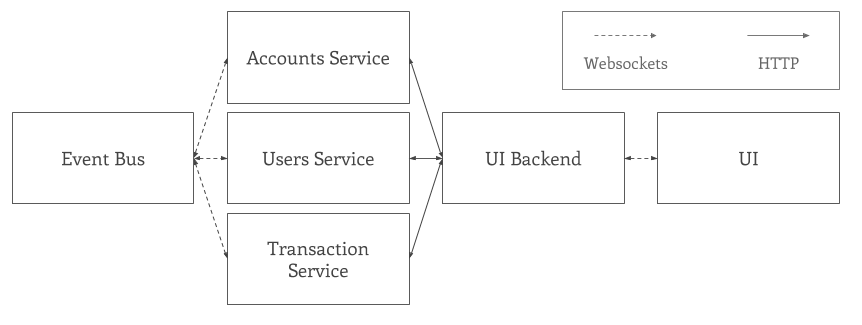
\includegraphics[width=15cm]{figures/microservices}
\end{center}
\caption{Microservices Architecture}
\label{fig:microservices}
\end{figure}

\subsection{Design}
Write something here!

\subsection{Initial Implementation}
Write something here!

\subsection{Superclient}
While the initial implementation of the microservices in Java worked and was reliable, it had various downsides that led to slowed iteration:

\begin{itemize}
    \item While each service did depend on the client library (also written in Java), due to the nature of the client library's design, implementations of many features - such as consistency, ACKs, and querying - would require many changes to the clients themselves. This resulted in a major slowdown to the time required to roll-out new features and test ideas, if the number of services was to increase, this slowdown would also increase.
    \item Services were hard to build. Due to the verbosity of Java and the functionality required by each service - namely a HTTP server with REST endpoints; and some variety of persistent storage - each service was quite large. If a new type of service was envisioned to supplement the other services or test an edge case in the implementation of other features, it would not have been practical to build due to time constraints.
\end{itemize}

For these reasons, an experimental project was started that would replace all of the clients and the client library with a framework for building microservices. This framework would handle all the necessary components required by a service - an event bus connection; a webserver; persistent storage - and delegate all processing or handling of events and requests to a scripting language that handles only the changing business logic of each service.

Dubbed the superclient, this project was written in Rust and took advantage of the team's existing knowledge from working on the event bus and allowed for code re-use through a shared common library between the projects. This common library also contained the schemas used to validate the JSON messages - by using the same schemas, we ensured that the superclient and event bus would always send valid JSON to each other.

It was decided that the superclient embed Lua to allow for the swappable service scripts. A minimal interface was exposed to Lua, where events could be sent and callbacks could be registered for new events, receipts for sent events and for rebuilding the state after downtime. Further, two functions were provided that would allow the services to query and fetch from a Redis key value store, enabling each type of service persistence. Other helper functions such as logging were also included.

After a handful of weeks in development, the superclient was ready to replace the existing Java infrastructure. In production, the services demonstrated the same reliability and conversion from the existing Java applications to small Lua scripts was quick and painless (typically taking only a day compared to the one-to-two weeks a Java service took to develop) - demonstrating the ease of use and rapid development enabled by the superclient.

Further, the superclient was easier to maintain - while an imperfect metric, the superclient was around 1700 lines of Rust code, and each service between 100-200 lines of Lua - this is a stark constrast to the Java applications, where the client library clocked in at 1800 lines of Java code, and each service between 600-800 lines. This far reduced the surface area for bugs and the amount of code that each team member would need to understand to work productively on the services.

This experimentation embodies one of the core ideas of the development team - if a team member can think of a way to improve the way something is done or implemented, then do it. This philosophy allowed the team to iterate quickly and not get bogged down with previous work that was unsuitable for current requirements.

%==============================================================================
\section{UI Backend}
\label{sec:backend}
Write something here!

\subsection{Design}
When deciding how the information was going to be sourced for the UI, there were two conflicting approaches discussed and debated. The first advocated for the UI backend to act as its own service, speaking directly to the event bus and not interacting with any of the microservices - which act as processing nodes only. Alternatively, the second approach advocated for the UI backend to speak only to the microservices through their REST APIs and never to the event bus directly.

The second approach would allow for the UI backend to query the internal state maintained by the services, reducing the processing required to build that state up itself from events directly. This would result in a faster, more responsive UI and was therefore chosen.

\subsection{Implementation}
Write something here!

%==============================================================================
\section{React}
\label{sec:react}
Write something here!

%==============================================================================
\section{Rust}
\label{sec:rust}
Write something here - touch on why, the frameworks used, the ecosystem.

%------------------------------------------------------------------------------
\section{Conclusions}
\label{sec:conclusions}

Explain the wider lessons that you learned about software engineering,
based on the specific issues discussed in previous sections.  Reflect
on the extent to which these lessons could be generalised to other
types of software project.  Relate the wider lessons to others
reported in case studies in the software engineering literature.

%------------------------------------------------------------------------------
\addcontentsline{toc}{section}{References}
\bibliographystyle{plain}
\bibliography{dissertation}

\end{document}
